\chapter{Results} \label{sec:results}
In this chapter we present the results of open-circuit simulations of the digital transformer.
An open circuit of a transformer is of particular interest, as it is generally used to determine core losses. 
We run the simulations for both the linear- as well as the non-linear model. 
All simulations are run with 
\begin{itemize}
    \item $I_s = 777.72$ A
    \item $I_p = 0$ A
    \item $N_s = 266$
    \item $N_p = 6$
    \item $f = 50$ Hz
\end{itemize}

\section{Linear behaviour}
Taking $\mu_{r, core} = 1000 \frac{\text{H}}{\text{m}}$  and $\mu_{r, air} = 10 \frac{\text{H}}{\text{m}}$ 
Figure \ref{fig:linear_model} shows the magnetic flux through all three core legs for several periods of the source signal
\begin{figure}[H]
    \centering
    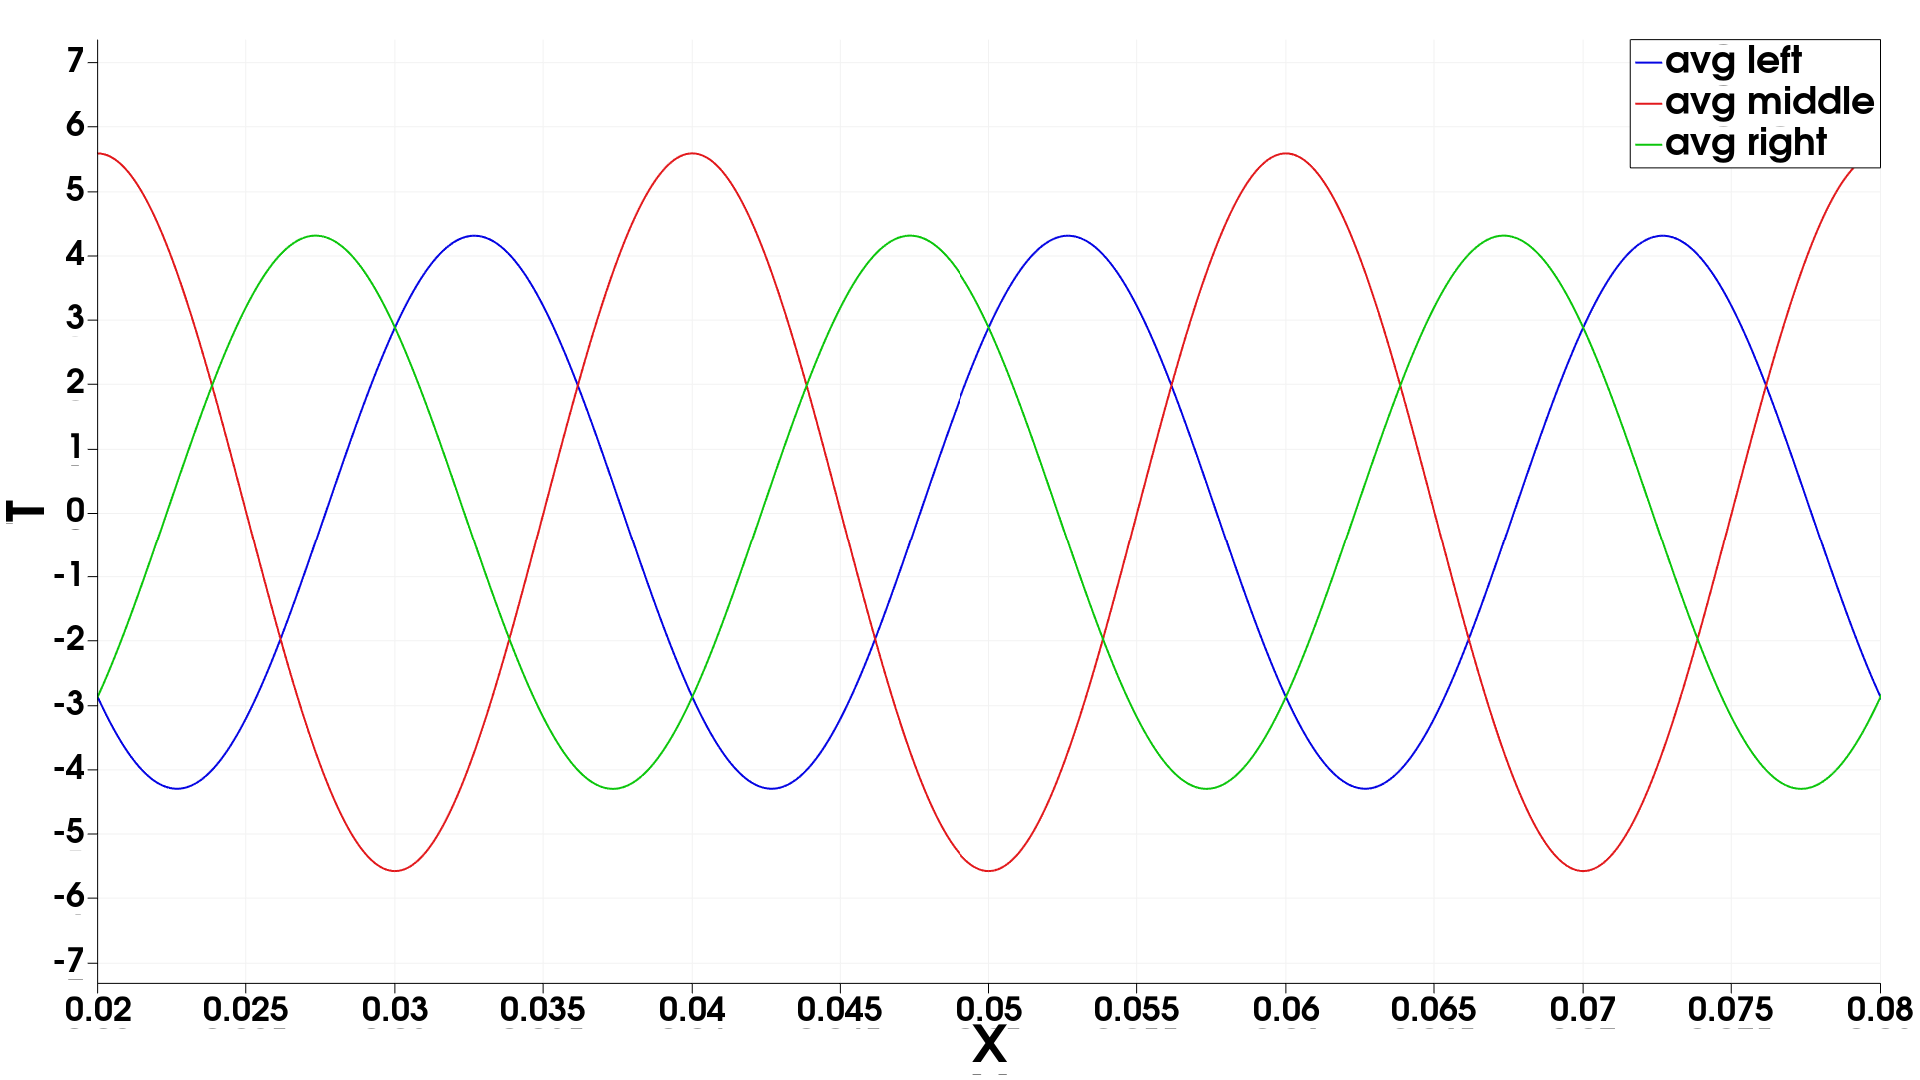
\includegraphics[width=0.8\textwidth]{img/B_phase_plot_linear_mu.png}
    \caption{Magnetic flux against time in all three core legs for the linear model.}
    \label{fig:linear_model}
\end{figure}
We can view this result as the superposition of three contributions, one for each core leg
\begin{align*}
    B_{\text{left leg}} &= B_0\left(\sin(\omega t - \phi) - \sin(\omega t)\right), \\
    B_{\text{middle leg}} &= B_0\left(\sin(\omega t) - \sin(\omega t - \phi) - \sin(\omega t + \phi)\right), \\
    B_{\text{right leg}} &= B_0\left(\sin(\omega t + \phi) - \sin(\omega t)\right),
\end{align*}
where $B_0$ is the amplitude of the magnetic flux and $\phi$ is the phase shift of the three-phase source signal.
Note that this is only true for the linear model. The above equations are derived by realising that any
coil induces a magnetic flux in the core leg it is wrapped around and an opposing flux in its neighbouring legs. Plotting above 
expressions gives Figure \ref{fig:linear_model_theory}.
\begin{figure}[H]
    \centering
    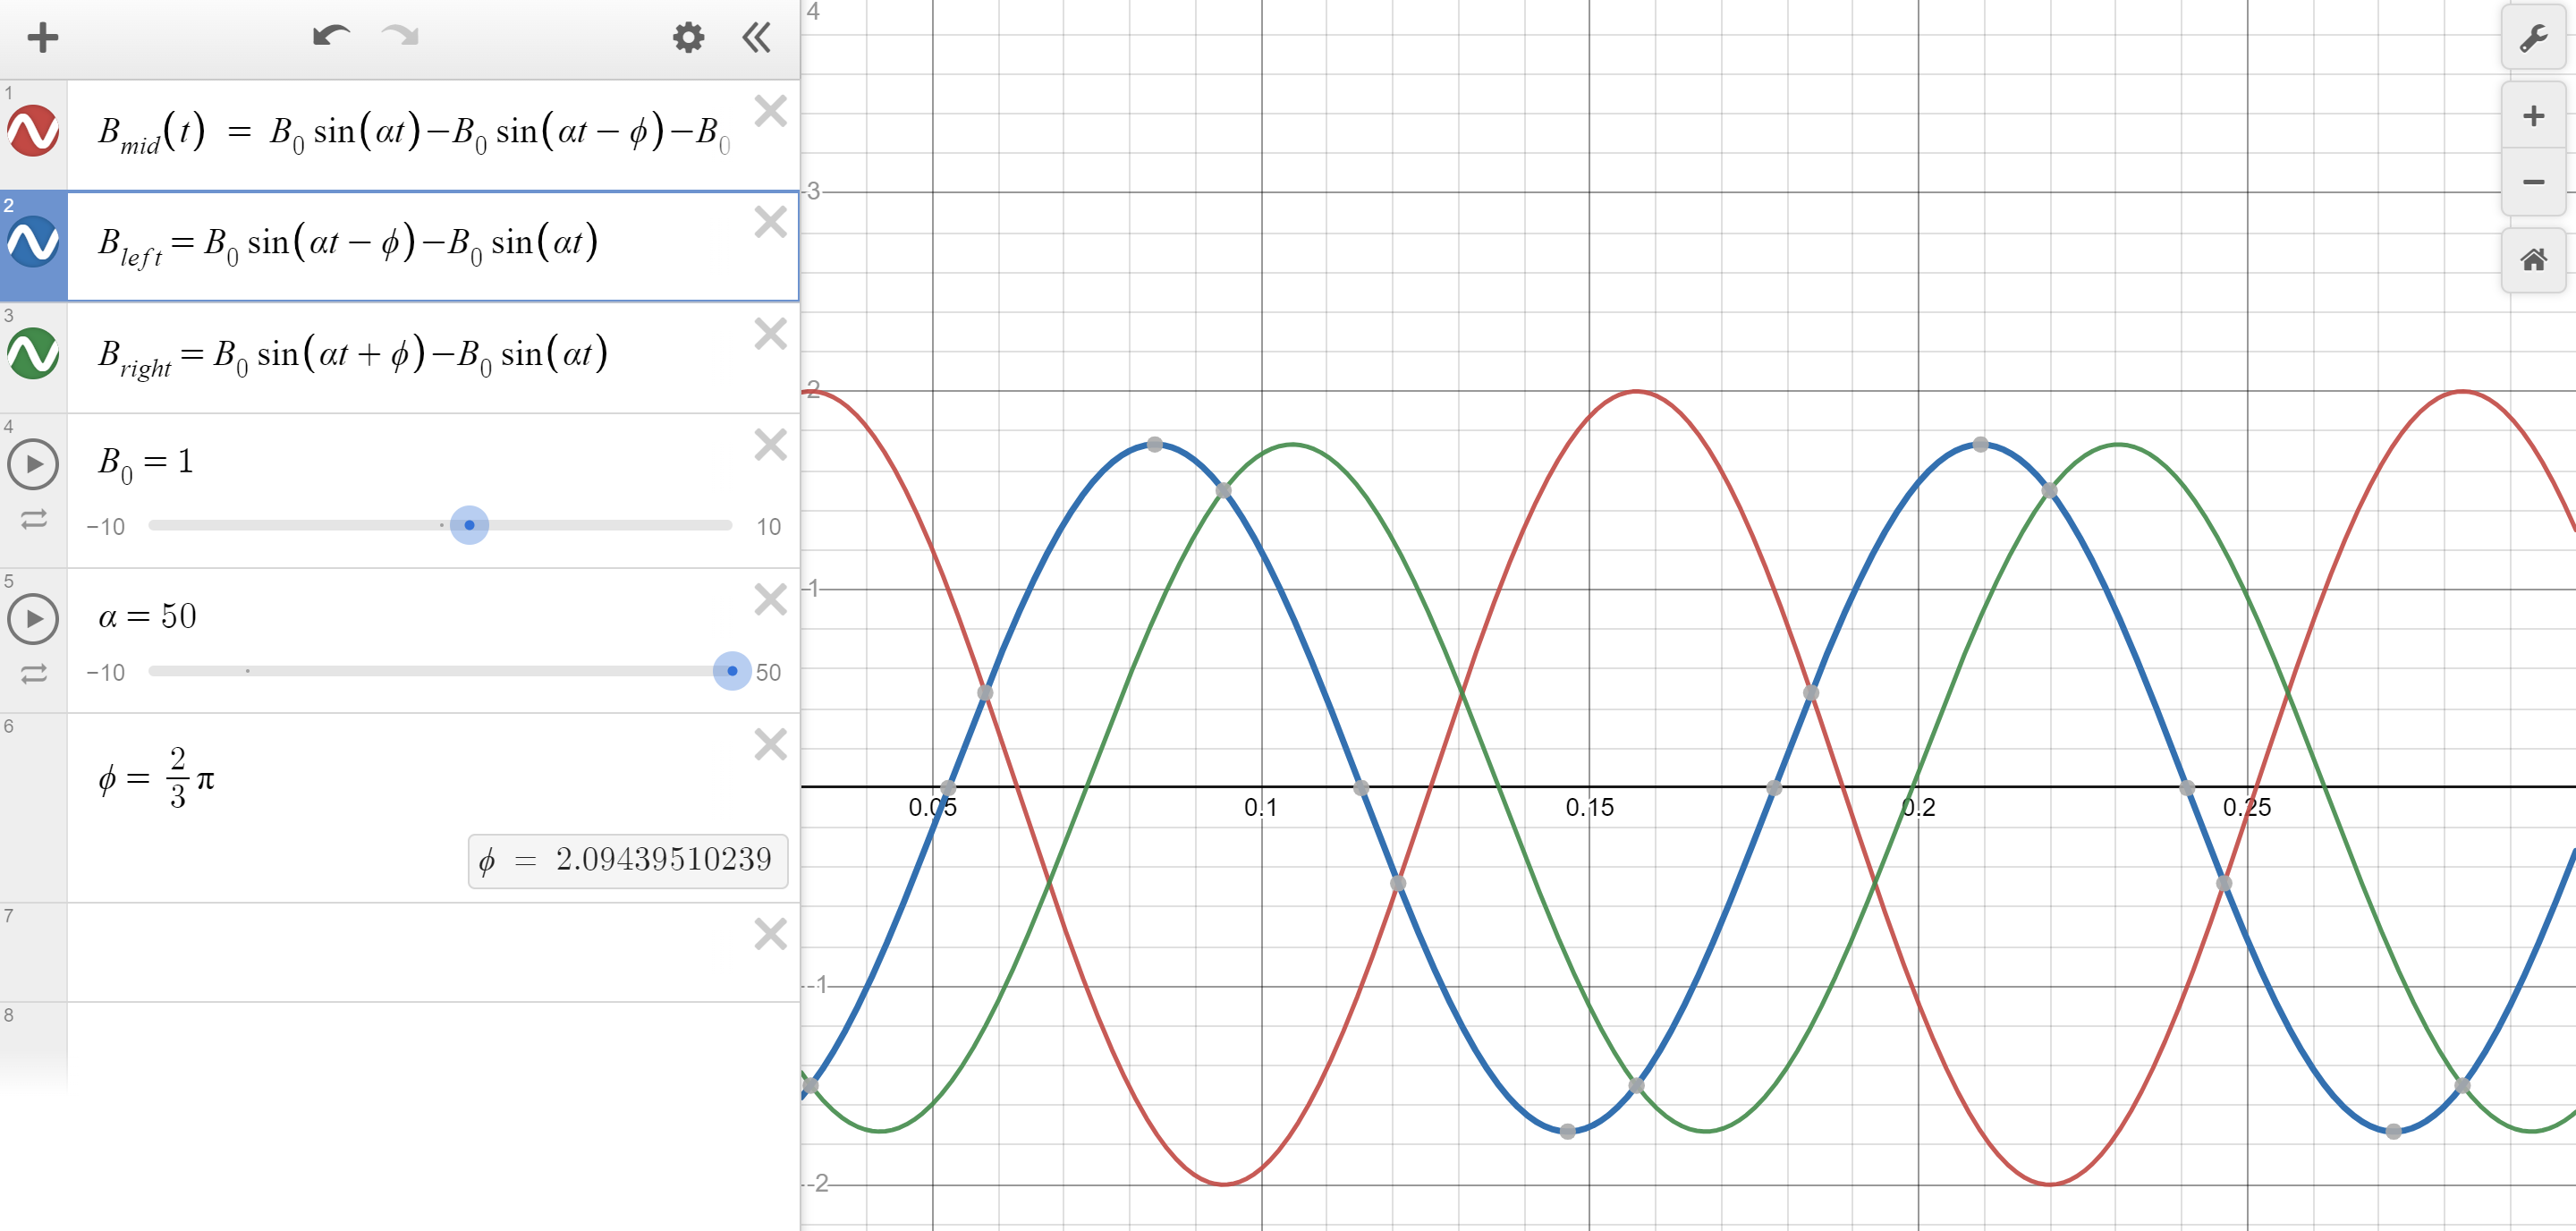
\includegraphics[width=0.8\textwidth]{img/Screenshot_68.png}
    \caption{Predicted magnetic flux against time in all three core legs for the linear model.}
    \label{fig:linear_model_theory}
\end{figure}

\section{Non-linear behaviour}
We now take 
\begin{equation*}
\mu_{\text{core, r}}(||\textbf{B}||) = \left(\alpha + (1 - \alpha) \frac{||\textbf{B}||^{2\beta}}{||\textbf{B}||^{2\beta} + \gamma}\right)^{-1},
\end{equation*}
$\alpha = 2.12 \times 10^{-4}$, $\beta = 7.358$ and $\gamma = 1.18 \times 10^{-4}$.
which has a saturation point at $||\textbf{B}|| \approx 2$ T.
Figure \ref{fig:nonlinear_phaseplot} shows the phase plot of $B$ for the non-linear model.
\begin{figure}[t]
    \centering
    \includegraphics[width=0.8\textwidth]{phaseplot_b_nonlinear.eps}
    \caption{Phase plot of $B$ for the non-linear model.}
    \label{fig:nonlinear_phaseplot}
\end{figure}
Note that the saturation points is clearly visible in the phase plot. Especially in the middle leg, where the magnetic flux is the highest.

The full solution for the magnetic flux in all three core legs is shown in Figure \ref{fig:nonlinear_bnorm}.
\begin{figure}[t]
    \centering
    \includegraphics[width=0.8\textwidth]{bnorm_t0.004.eps}
    \caption{Bnorm for the non-linear model.}
    \label{fig:nonlinear_bnorm}
\end{figure}
This phase plot is more complex than the combination of three sinusoidal functions, which sets the linear model apart from the non-linear model.
Another area where we see differences between the linear and non-linear model is the permeability. The latter is shown in Figure \ref{fig:nonlinear_permeability}.
\begin{figure}[t]
    \centering
    \includegraphics[width=0.8\textwidth]{permeability_t0.004.eps}
    \caption{Permeability for the non-linear model.}
    \label{fig:nonlinear_permeability}
\end{figure}
Figure \ref{fig:nonlinear_permeability_bnorm} shows the permeability as a function of $||B||$.
\begin{figure}[t]
    \centering
    \includegraphics[width=0.8\textwidth]{permeability_nonlinear.eps}
    \caption{Permeability as a function of $||B||$.}
    \label{fig:nonlinear_permeability_bnorm}
\end{figure}





